本节与拓展 A 共用同一组批次：8:00、13:00、18:00、23:00 各随机抽取 5 个批次，每批 40 个司机、80 个订单，距离量化到 10\,m。每个批次先用 \cref{sec:exact} 的方法求出精确前沿 $Z^\ast$，作为真值。三种进化算法各运行 5 个种子，加权和 KM 是确定性方法，只运行一次。所有指标都以 $Z^\ast$ 的理想点和最差点归一化：HV 比为 $\mathrm{HV}/\mathrm{HV}^\ast$，IGD 与 IGD$^+$ 越小越好，“命中率”指近似解中恰好落在 $Z^\ast$ 上的比例。

\begin{figure}[t]
	\centering
	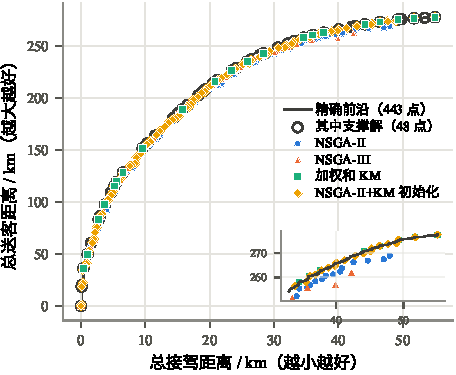
\includegraphics[width=\columnwidth]{fig/exp2_front.pdf}
	\caption{18:00 代表批次的帕累托前沿（右下为高收入端放大）。空心圆为精确前沿上的支撑解}
	\label{fig:front}
\end{figure}

\textbf{前沿形状与折中解。} \Cref{fig:front} 中，前沿在低接驾端很陡、在高收入端很平，边际收益递减明显。以与两端点连线距离最远的点（膝点）为折中方案，20 个批次平均只需最大接驾距离的 31.6\%，就能获得最大送客距离的 71.1\%。这说明平台若完全追求收入最大化，最后约 29\% 的收入需要付出约 68\% 的额外接驾距离。

\begin{table}[t]
	\centering
	\caption{近似算法对比（20 批次 × 5 种子均值；末列为以 IGD$^+$ 计的 Friedman 平均秩）}
	\label{tab:moo}
	\resizebox{\columnwidth}{!}{%
	\begin{tabular}{lccccccc}
		\toprule
		方法 & HV 比$\uparrow$ & IGD$\downarrow$ & IGD$^+\downarrow$ & Spacing$\downarrow$ & 解数 & 命中率/\% & 秩 \\
		\midrule
		\tabinput{tables/exp24_methods.tex}
		\bottomrule
	\end{tabular}}
\end{table}

\begin{figure}[t]
	\centering
	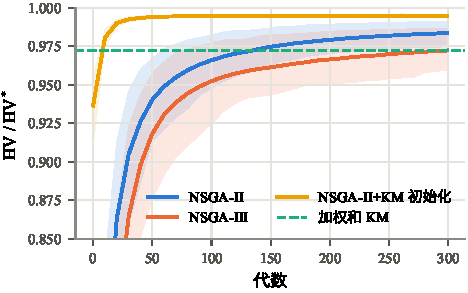
\includegraphics[width=\columnwidth]{fig/exp2_convergence.pdf}
	\caption{HV 比随代数的收敛（100 条曲线的均值，阴影为 10\%–90\% 分位）}
	\label{fig:conv}
\end{figure}

\textbf{算法比较。} 由\cref{tab:moo} 和\cref{fig:conv} 可以得到三点结论。(1) 两个目标时，NSGA-II 明显优于 NSGA-III：HV 比为 0.984 对 0.972，Spacing 为 0.47 对 0.84。NSGA-III 的参考方向在归一化目标空间中按角度均匀分布，而本问题的前沿弯曲程度很大，解会集中在少数方向上，拥挤距离反而能更好地适应局部密度。(2) 加权和 KM 每次都解到真正的最优，命中率达 98.9\%（未命中的点来自 $\lambda=0$ 时只最大化收入、接驾距离不唯一的弱支配解）。但它平均只找到 21.4 个点，HV 比仅 0.972，IGD$^+$ 是各方法中最差的。(3) KM 初始化把加权和 KM 的精确解作为“锚点”，NSGA-II 在锚点之间继续搜索非支撑解。这一做法使 HV 比提高到 0.995，IGD$^+$ 从 0.0071 降到 0.0033（约 54\%），命中率从 31\% 升到 55\%，并且在第 20 代左右就超过随机初始化 300 代的水平。

\textbf{统计检验。} 以 20 个批次为区组、IGD$^+$ 为指标做 Friedman 检验，$p=2.9\times10^{-11}$。四种方法的平均秩依次为 KM 初始化 1.0、NSGA-II 2.1、NSGA-III 3.2、加权和 3.7。Nemenyi 临界差 CD $=1.05$（$\alpha=0.05$），因此前三者两两之间差异显著，NSGA-III 与加权和之间不显著。配对 Wilcoxon 检验得到相同结论：KM 初始化对 NSGA-II，以及 NSGA-II 对加权和，均有 $p<10^{-5}$。

\subsection{拓展实验 A：精确前沿揭示的结构}

\begin{figure}[t]
	\centering
	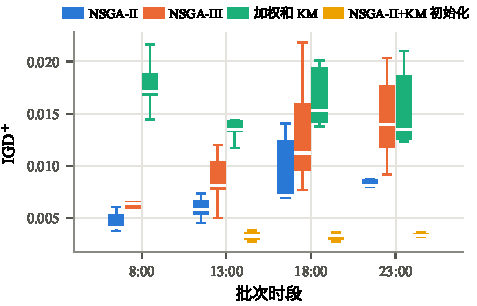
\includegraphics[width=\columnwidth]{fig/exp4_igd_hour.pdf}
	\caption{不同时段批次上各方法的 IGD$^+$（越小越好；每箱 5 个批次，每批取 5 个种子均值）}
	\label{fig:igdhour}
\end{figure}

20 个批次的精确前沿全部通过了 \cref{sec:exact} 中的逐点验证，修复次数为 0。每个批次平均有 445 个非支配点（306–593 个），平均需要求解 1335 次整数规划，点数最多的批次（593 点）在单进程下约需 3.4 分钟。主要发现如下：

\textbf{(1) 帕累托前沿以非支撑解为主。} 位于下凸包上的支撑解平均只有 43.5 个，占 \textbf{10.0\%}（各批次在 8.0\%–14.4\% 之间）。任何线性加权方法，无论 $\lambda$ 取得多密，都只能覆盖这约 10\% 的点。离散匹配问题的可行组合非常多，相邻的支撑解之间分布着大量“凹陷处”的折中解，这正是进化算法相对加权和方法的优势所在。此前的作业只把 HV 比作为评价依据，加权和 KM 与 NSGA-II 的 HV 比只差约 0.01，看起来接近。有了精确前沿，可以确认两者的差距真实存在，主要体现在前沿的覆盖率上（IGD$^+$ 相差 2.2 倍）。

\textbf{(2) 难度随时段变化。} \Cref{fig:igdhour} 中，18:00 和 23:00 批次的可行订单更多（平均 63 和 71 单，8:00 与 13:00 均约 59 单），前沿点更多，随机初始化的 NSGA-II/III 误差明显增大。KM 初始化在四个时段上的 IGD$^+$ 都稳定在 0.003 左右，对问题规模不敏感。

\textbf{(3) 对作业中“竞争比”的补充。} 若以精确前沿为基准，NSGA-II 找到的最高送客距离平均为 269.3\,km，比真实最大值 278.5\,km 低 3.3\%；而 KM 初始化与加权和 KM 都能达到真实最大值。可见随机初始化的进化算法在前沿两端收敛不足，用精确解作锚点可以弥补这一点。
